\documentclass[]{book}
\usepackage{lmodern}
\usepackage{amssymb,amsmath}
\usepackage{ifxetex,ifluatex}
\usepackage{fixltx2e} % provides \textsubscript
\ifnum 0\ifxetex 1\fi\ifluatex 1\fi=0 % if pdftex
  \usepackage[T1]{fontenc}
  \usepackage[utf8]{inputenc}
\else % if luatex or xelatex
  \ifxetex
    \usepackage{mathspec}
  \else
    \usepackage{fontspec}
  \fi
  \defaultfontfeatures{Ligatures=TeX,Scale=MatchLowercase}
\fi
% use upquote if available, for straight quotes in verbatim environments
\IfFileExists{upquote.sty}{\usepackage{upquote}}{}
% use microtype if available
\IfFileExists{microtype.sty}{%
\usepackage{microtype}
\UseMicrotypeSet[protrusion]{basicmath} % disable protrusion for tt fonts
}{}
\usepackage[margin=1in]{geometry}
\usepackage{hyperref}
\hypersetup{unicode=true,
            pdftitle={R for Research},
            pdfauthor={Abhay Singh},
            pdfborder={0 0 0},
            breaklinks=true}
\urlstyle{same}  % don't use monospace font for urls
\usepackage{natbib}
\bibliographystyle{apalike}
\usepackage{color}
\usepackage{fancyvrb}
\newcommand{\VerbBar}{|}
\newcommand{\VERB}{\Verb[commandchars=\\\{\}]}
\DefineVerbatimEnvironment{Highlighting}{Verbatim}{commandchars=\\\{\}}
% Add ',fontsize=\small' for more characters per line
\usepackage{framed}
\definecolor{shadecolor}{RGB}{248,248,248}
\newenvironment{Shaded}{\begin{snugshade}}{\end{snugshade}}
\newcommand{\KeywordTok}[1]{\textcolor[rgb]{0.13,0.29,0.53}{\textbf{#1}}}
\newcommand{\DataTypeTok}[1]{\textcolor[rgb]{0.13,0.29,0.53}{#1}}
\newcommand{\DecValTok}[1]{\textcolor[rgb]{0.00,0.00,0.81}{#1}}
\newcommand{\BaseNTok}[1]{\textcolor[rgb]{0.00,0.00,0.81}{#1}}
\newcommand{\FloatTok}[1]{\textcolor[rgb]{0.00,0.00,0.81}{#1}}
\newcommand{\ConstantTok}[1]{\textcolor[rgb]{0.00,0.00,0.00}{#1}}
\newcommand{\CharTok}[1]{\textcolor[rgb]{0.31,0.60,0.02}{#1}}
\newcommand{\SpecialCharTok}[1]{\textcolor[rgb]{0.00,0.00,0.00}{#1}}
\newcommand{\StringTok}[1]{\textcolor[rgb]{0.31,0.60,0.02}{#1}}
\newcommand{\VerbatimStringTok}[1]{\textcolor[rgb]{0.31,0.60,0.02}{#1}}
\newcommand{\SpecialStringTok}[1]{\textcolor[rgb]{0.31,0.60,0.02}{#1}}
\newcommand{\ImportTok}[1]{#1}
\newcommand{\CommentTok}[1]{\textcolor[rgb]{0.56,0.35,0.01}{\textit{#1}}}
\newcommand{\DocumentationTok}[1]{\textcolor[rgb]{0.56,0.35,0.01}{\textbf{\textit{#1}}}}
\newcommand{\AnnotationTok}[1]{\textcolor[rgb]{0.56,0.35,0.01}{\textbf{\textit{#1}}}}
\newcommand{\CommentVarTok}[1]{\textcolor[rgb]{0.56,0.35,0.01}{\textbf{\textit{#1}}}}
\newcommand{\OtherTok}[1]{\textcolor[rgb]{0.56,0.35,0.01}{#1}}
\newcommand{\FunctionTok}[1]{\textcolor[rgb]{0.00,0.00,0.00}{#1}}
\newcommand{\VariableTok}[1]{\textcolor[rgb]{0.00,0.00,0.00}{#1}}
\newcommand{\ControlFlowTok}[1]{\textcolor[rgb]{0.13,0.29,0.53}{\textbf{#1}}}
\newcommand{\OperatorTok}[1]{\textcolor[rgb]{0.81,0.36,0.00}{\textbf{#1}}}
\newcommand{\BuiltInTok}[1]{#1}
\newcommand{\ExtensionTok}[1]{#1}
\newcommand{\PreprocessorTok}[1]{\textcolor[rgb]{0.56,0.35,0.01}{\textit{#1}}}
\newcommand{\AttributeTok}[1]{\textcolor[rgb]{0.77,0.63,0.00}{#1}}
\newcommand{\RegionMarkerTok}[1]{#1}
\newcommand{\InformationTok}[1]{\textcolor[rgb]{0.56,0.35,0.01}{\textbf{\textit{#1}}}}
\newcommand{\WarningTok}[1]{\textcolor[rgb]{0.56,0.35,0.01}{\textbf{\textit{#1}}}}
\newcommand{\AlertTok}[1]{\textcolor[rgb]{0.94,0.16,0.16}{#1}}
\newcommand{\ErrorTok}[1]{\textcolor[rgb]{0.64,0.00,0.00}{\textbf{#1}}}
\newcommand{\NormalTok}[1]{#1}
\usepackage{longtable,booktabs}
\usepackage{graphicx,grffile}
\makeatletter
\def\maxwidth{\ifdim\Gin@nat@width>\linewidth\linewidth\else\Gin@nat@width\fi}
\def\maxheight{\ifdim\Gin@nat@height>\textheight\textheight\else\Gin@nat@height\fi}
\makeatother
% Scale images if necessary, so that they will not overflow the page
% margins by default, and it is still possible to overwrite the defaults
% using explicit options in \includegraphics[width, height, ...]{}
\setkeys{Gin}{width=\maxwidth,height=\maxheight,keepaspectratio}
\IfFileExists{parskip.sty}{%
\usepackage{parskip}
}{% else
\setlength{\parindent}{0pt}
\setlength{\parskip}{6pt plus 2pt minus 1pt}
}
\setlength{\emergencystretch}{3em}  % prevent overfull lines
\providecommand{\tightlist}{%
  \setlength{\itemsep}{0pt}\setlength{\parskip}{0pt}}
\setcounter{secnumdepth}{5}
% Redefines (sub)paragraphs to behave more like sections
\ifx\paragraph\undefined\else
\let\oldparagraph\paragraph
\renewcommand{\paragraph}[1]{\oldparagraph{#1}\mbox{}}
\fi
\ifx\subparagraph\undefined\else
\let\oldsubparagraph\subparagraph
\renewcommand{\subparagraph}[1]{\oldsubparagraph{#1}\mbox{}}
\fi

%%% Use protect on footnotes to avoid problems with footnotes in titles
\let\rmarkdownfootnote\footnote%
\def\footnote{\protect\rmarkdownfootnote}

%%% Change title format to be more compact
\usepackage{titling}

% Create subtitle command for use in maketitle
\newcommand{\subtitle}[1]{
  \posttitle{
    \begin{center}\large#1\end{center}
    }
}

\setlength{\droptitle}{-2em}

  \title{R for Research}
    \pretitle{\vspace{\droptitle}\centering\huge}
  \posttitle{\par}
    \author{Abhay Singh}
    \preauthor{\centering\large\emph}
  \postauthor{\par}
      \predate{\centering\large\emph}
  \postdate{\par}
    \date{2019-02-04}

\usepackage{booktabs}
\usepackage{amsthm}
\makeatletter
\def\thm@space@setup{%
  \thm@preskip=8pt plus 2pt minus 4pt
  \thm@postskip=\thm@preskip
}
\makeatother

\begin{document}
\maketitle

{
\setcounter{tocdepth}{1}
\tableofcontents
}
\chapter{Preface}\label{preface}

This is a compilcation of handouts for \emph{\(R^2: R for Research\)}
written in \textbf{Markdown}. Y

ou can use anything that Pandoc's Markdown supports, e.g., a math
equation \(a^2 + b^2 = c^2\).

The \textbf{bookdown} package can be installed from CRAN or Github:

\begin{Shaded}
\begin{Highlighting}[]
\KeywordTok{install.packages}\NormalTok{(}\StringTok{"bookdown"}\NormalTok{)}
\CommentTok{# or the development version}
\CommentTok{# devtools::install_github("rstudio/bookdown")}
\end{Highlighting}
\end{Shaded}

Remember each Rmd file contains one and only one chapter, and a chapter
is defined by the first-level heading \texttt{\#}.

To compile this example to PDF, you need XeLaTeX. You are recommended to
install TinyTeX (which includes XeLaTeX):
\url{https://yihui.name/tinytex/}.

\chapter{What is R?}\label{what-is-r}

According to the official webpage:

\begin{itemize}
\tightlist
\item
  R is a language and environment for statistical computing and
  graphics. It is a GNU project which is similar to the S language and
  environment which was developed at Bell Laboratories (formerly AT\&T,
  now Lucent Technologies) by John Chambers and colleagues. R can be
  considered as a different implementation of S. There are some
  important differences, but much code written for S runs unaltered
  under R. \url{http://www.r-project.org/about.html}
\end{itemize}

\emph{According to Wikipedia}

\begin{itemize}
\tightlist
\item
  R is a free software programming language and a software environment
  for statistical computing and graphics. The R language is widely used
  among statisticians and data miners for developing statistical
  software and data analysis. Polls and surveys of data miners are
  showing R's popularity has increased substantially in recent years.
\end{itemize}

To Summarise

\begin{itemize}
\item
  R is the most amazing free statistical software ever!
\item
  This recent video by Revolution Analytics does a great job in
  summarizing R
\end{itemize}

!

\section{Why should we learn R?}\label{why-should-we-learn-r}

R follows a type inference \footnote{Type inference refers to the
  automatic deduction of the type of an expression in a programming
  language.} coding structure and provides a wide variety of statistical
and graphical techniques, including;

\begin{quote}
\begin{itemize}
\tightlist
\item
  Linear and non-linear modelling
\end{itemize}
\end{quote}

\begin{quote}
\begin{itemize}
\tightlist
\item
  Univariate \& Multivariate Statistics
\end{itemize}
\end{quote}

\begin{quote}
\begin{itemize}
\tightlist
\item
  Classical statistical tests
\end{itemize}
\end{quote}

\begin{quote}
\begin{itemize}
\tightlist
\item
  Time-series analysis/ Econometrics
\end{itemize}
\end{quote}

\begin{quote}
\begin{itemize}
\tightlist
\item
  Simulation and Modelling
\end{itemize}
\end{quote}

\begin{quote}
\begin{itemize}
\tightlist
\item
  Datamining-classification, clustering etc.
\end{itemize}
\end{quote}

\begin{quote}
\begin{itemize}
\tightlist
\item
  For computationally intensive tasks, C, C++, and Fortran code can be
  linked and called at run time.
\end{itemize}
\end{quote}

\begin{quote}
\begin{itemize}
\tightlist
\item
  R is easily extensible through functions and extensions, and the R
  community is noted for its active contributions in terms of packages.
\end{itemize}
\end{quote}

\begin{Shaded}
\begin{Highlighting}[]
\CommentTok{#Number of R Packages }
\KeywordTok{length}\NormalTok{(}\KeywordTok{available.packages}\NormalTok{(}\DataTypeTok{repos =} \StringTok{"http://cran.us.r-project.org"}\NormalTok{)[,}\DecValTok{1}\NormalTok{])}
\end{Highlighting}
\end{Shaded}

\begin{verbatim}
## [1] 13636
\end{verbatim}

\begin{itemize}
\tightlist
\item
  Total 13636 packages and counting
\end{itemize}

\section{Installing R and RStudio on Windows}\label{Rinstall}

\begin{itemize}
\item
  The latest version of R can be download from the R homepage.
\item
  R download page: \url{http://www.cran.r-project.org/bin/windows/base/}
  The page also provides some instructions and FAQ's on R installation.
\item
  RStudio IDE ( \emph{IDE: Integrated Development Environment}) is a
  powerful and productive user interface for R.
\item
  It's free and open source, and works great on Windows, Mac, and Linux
\end{itemize}

\section{RStudio GUI/IDE}\label{rstudio-guiide}

\begin{itemize}
\item
  RStudio GUI is composed of 4 panes which can be rearranged according
  to the requirements.
\item
  There are a lot of short introductions to RStudio available online so
  we will not go into more details.
\end{itemize}

The figure below gives the snapshot of RStudio GUI.

\begin{figure}
\centering
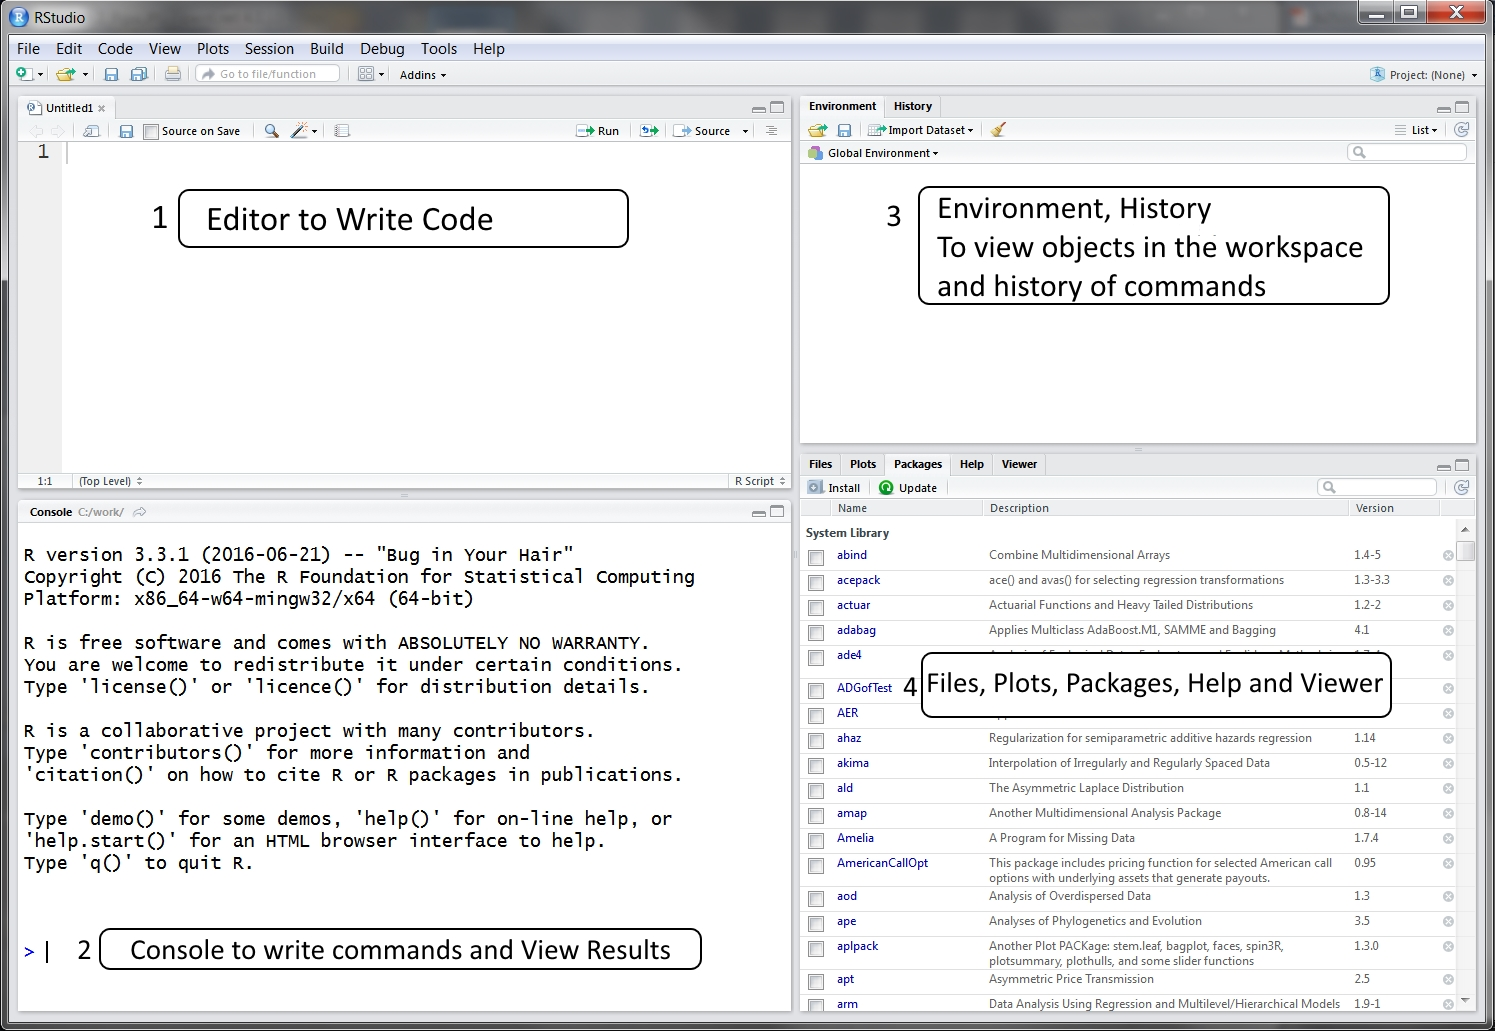
\includegraphics{Figure-1.2-RStudio.jpg}
\caption{\label{fig:unnamed-chunk-2}RStudio IDE}
\end{figure}

\begin{itemize}
\tightlist
\item
  A short intro to RStudio !

  RStudio Overview - 1:30 from RStudio, Inc. on Vimeo.
\end{itemize}

\section{Installing Packages}\label{installing-packages}

\begin{itemize}
\item
  The easiest way to install packages is to do it via R console. The
  command install.packages(``package name'') installs R packages
  directly from internet. Other options to install various dependencies
  to a package can be easily specified when calling this function. A
  call to this function asks the user to chose a CRAN mirror at the
  first instance.
\item
  Run the following to install Quantreg package on R. Also use the help
  function to get the details.
\end{itemize}

\begin{Shaded}
\begin{Highlighting}[]
\CommentTok{#Install a package using RStudio Console}
\KeywordTok{install.packages}\NormalTok{(}\StringTok{"quantreg"}\NormalTok{,}\DataTypeTok{dependencies=}\KeywordTok{c}\NormalTok{(}\StringTok{"Depends"}\NormalTok{,}\StringTok{"Suggests"}\NormalTok{))}
\end{Highlighting}
\end{Shaded}

\begin{Shaded}
\begin{Highlighting}[]
\KeywordTok{install.packages}\NormalTok{(}\KeywordTok{c}\NormalTok{(}\StringTok{"zoo"}\NormalTok{,}\StringTok{"reshape2"}\NormalTok{,}\StringTok{"quantreg"}\NormalTok{,}\StringTok{"e1071"}\NormalTok{,}\StringTok{"foreign"}\NormalTok{,}\StringTok{"psych"}\NormalTok{,}\StringTok{"pastecs"}\NormalTok{,}\StringTok{"ggplot2"}\NormalTok{,}\StringTok{"stargazer"}\NormalTok{,}\StringTok{"formatR"}\NormalTok{,}\StringTok{"plm"}\NormalTok{,}\StringTok{"xts"}\NormalTok{,}\StringTok{"tseries"}\NormalTok{,}\StringTok{"fArma"}\NormalTok{), }\DataTypeTok{dependencies =} \OtherTok{TRUE}\NormalTok{) }
\CommentTok{#to be updated}
\end{Highlighting}
\end{Shaded}

You can label chapter and section titles using \texttt{\{\#label\}}
after them, e.g., we can reference Chapter \ref{intro}. If you do not
manually label them, there will be automatic labels anyway, e.g.,
Chapter \ref{methods}.

Figures and tables with captions will be placed in \texttt{figure} and
\texttt{table} environments, respectively.

\begin{Shaded}
\begin{Highlighting}[]
\KeywordTok{par}\NormalTok{(}\DataTypeTok{mar =} \KeywordTok{c}\NormalTok{(}\DecValTok{4}\NormalTok{, }\DecValTok{4}\NormalTok{, .}\DecValTok{1}\NormalTok{, .}\DecValTok{1}\NormalTok{))}
\KeywordTok{plot}\NormalTok{(pressure, }\DataTypeTok{type =} \StringTok{'b'}\NormalTok{, }\DataTypeTok{pch =} \DecValTok{19}\NormalTok{)}
\end{Highlighting}
\end{Shaded}

\begin{figure}

{\centering 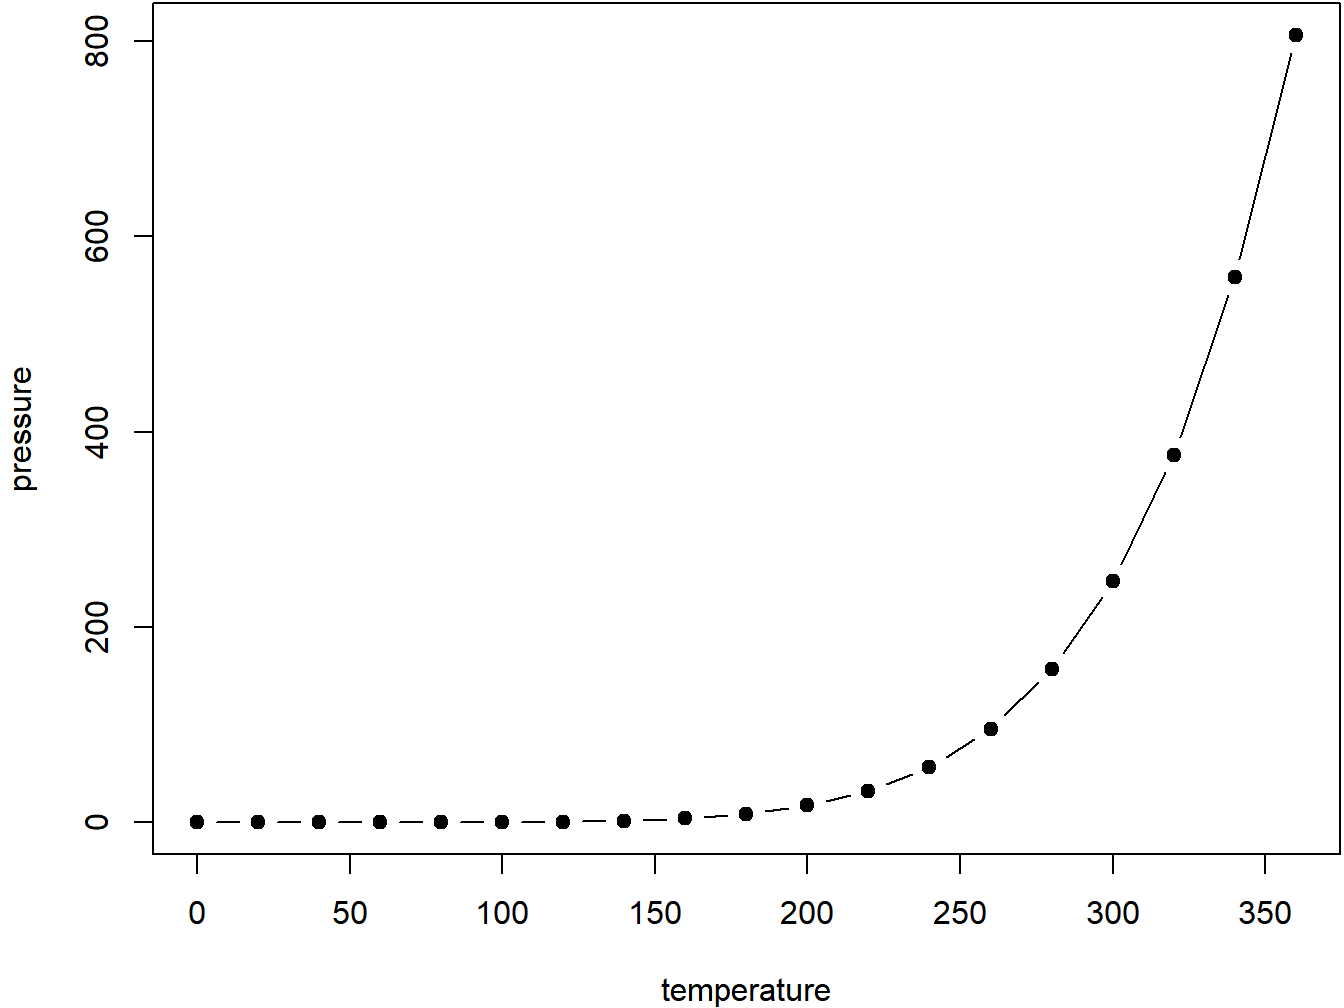
\includegraphics[width=0.8\linewidth]{01-intro_files/figure-latex/nice-fig-1} 

}

\caption{Here is a nice figure!}\label{fig:nice-fig}
\end{figure}

Reference a figure by its code chunk label with the \texttt{fig:}
prefix, e.g., see Figure \ref{fig:nice-fig}. Similarly, you can
reference tables generated from \texttt{knitr::kable()}, e.g., see Table
\ref{tab:nice-tab}.

\begin{Shaded}
\begin{Highlighting}[]
\NormalTok{knitr}\OperatorTok{::}\KeywordTok{kable}\NormalTok{(}
  \KeywordTok{head}\NormalTok{(iris, }\DecValTok{20}\NormalTok{), }\DataTypeTok{caption =} \StringTok{'Here is a nice table!'}\NormalTok{,}
  \DataTypeTok{booktabs =} \OtherTok{TRUE}
\NormalTok{)}
\end{Highlighting}
\end{Shaded}

\begin{table}[t]

\caption{\label{tab:nice-tab}Here is a nice table!}
\centering
\begin{tabular}{rrrrl}
\toprule
Sepal.Length & Sepal.Width & Petal.Length & Petal.Width & Species\\
\midrule
5.1 & 3.5 & 1.4 & 0.2 & setosa\\
4.9 & 3.0 & 1.4 & 0.2 & setosa\\
4.7 & 3.2 & 1.3 & 0.2 & setosa\\
4.6 & 3.1 & 1.5 & 0.2 & setosa\\
5.0 & 3.6 & 1.4 & 0.2 & setosa\\
\addlinespace
5.4 & 3.9 & 1.7 & 0.4 & setosa\\
4.6 & 3.4 & 1.4 & 0.3 & setosa\\
5.0 & 3.4 & 1.5 & 0.2 & setosa\\
4.4 & 2.9 & 1.4 & 0.2 & setosa\\
4.9 & 3.1 & 1.5 & 0.1 & setosa\\
\addlinespace
5.4 & 3.7 & 1.5 & 0.2 & setosa\\
4.8 & 3.4 & 1.6 & 0.2 & setosa\\
4.8 & 3.0 & 1.4 & 0.1 & setosa\\
4.3 & 3.0 & 1.1 & 0.1 & setosa\\
5.8 & 4.0 & 1.2 & 0.2 & setosa\\
\addlinespace
5.7 & 4.4 & 1.5 & 0.4 & setosa\\
5.4 & 3.9 & 1.3 & 0.4 & setosa\\
5.1 & 3.5 & 1.4 & 0.3 & setosa\\
5.7 & 3.8 & 1.7 & 0.3 & setosa\\
5.1 & 3.8 & 1.5 & 0.3 & setosa\\
\bottomrule
\end{tabular}
\end{table}

You can write citations, too. For example, we are using the
\textbf{bookdown} package \citep{R-bookdown} in this sample book, which
was built on top of R Markdown and \textbf{knitr} \citep{xie2015}.

\chapter{Methods}\label{methods}

We describe our methods in this chapter.

\chapter{Applications}\label{applications}

Some \emph{significant} applications are demonstrated in this chapter.

\section{Example one}\label{example-one}

\section{Example two}\label{example-two}

\chapter{Final Words}\label{final-words}

We have finished a nice book.

\bibliography{book.bib,packages.bib}


\end{document}
